\section{Experiments and Results}


All the test cases were divided in to 50\% base case and the remaining 50\% to iterations of 2.5\% (e.g. 20 iterations).

The implementation was done using Spark~\cite{spark}.

The used hardware is 4 clusters each with 20G memory and 40 cores. Also used SparkRDMA Plugin~\cite{SparkRDMA}.

For PFP~\cite{li2008pfp} performance comparison, Spark~\cite{spark} mllib package implements just that, and was used per iteration.

For CanTree~\cite{leung2005cantree} performance, we used IPFIM with only one group, meaning a single tree.

\subsection{PFP VS IPFIM}
 For correct PFP~\cite{li2008pfp} mining, a read of all the dataset till that point needs to be performed.

For the synthetic datasets, a comparison for minSup of 0.001 can be seen at \autoref{fig:PFPvsIPFP}. As seen, PFP~\cite{li2008pfp} starts better, but after a few iterations, IPFIM is more flat for every iteration, while PFP~\cite{li2008pfp} increases linearly.

For the Kosarak dataset, results are seen in \autoref{fig:PFPvsIPFPKos}.
Since there are much more frequent items for minSup of 0.001, the results show a poor performance for mining with only 10 partitions, since the trees are much larger. For 100 partitions, the results are still better for PFP~\cite{li2008pfp}, where the exponential mining process is the bottle neck for IPFIM. An improvment is discussed in section XXX

\begin{figure}
  \centering
  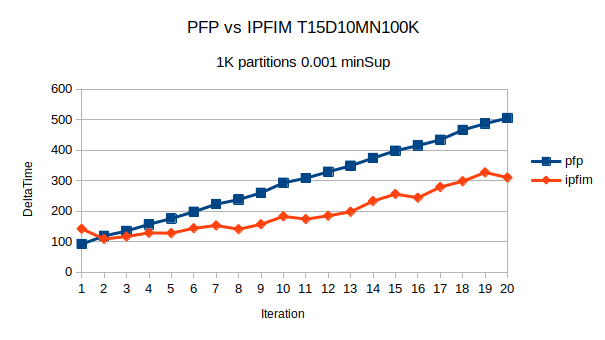
\includegraphics[width=\linewidth]{figures/PFPvsIPFIM0_001_10M}
  \caption{PFP vs IPFIM 10M}
  \label{fig:PFPvsIPFP}
\end{figure}

\begin{figure}
  \centering
  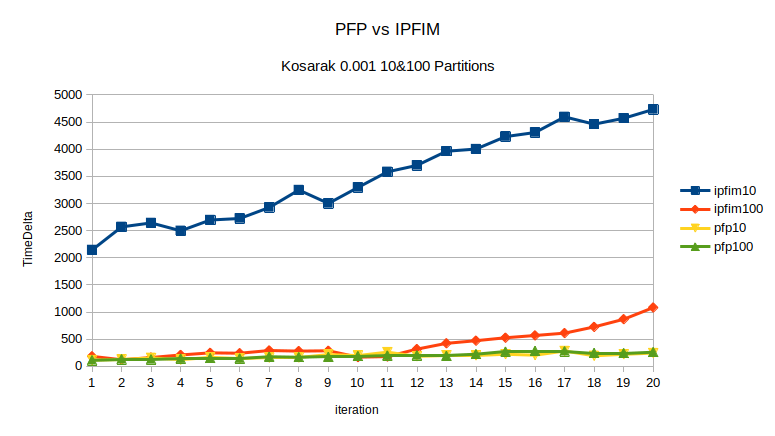
\includegraphics[width=\linewidth]{figures/PFPvsIPFIM0_001_Kosarak}
  \caption{PFP vs IPFIM Kosarak}
  \label{fig:PFPvsIPFPKos}
\end{figure}


\subsection{IPFIM vs Interactive CanTree}
\begin{figure}
  \centering
  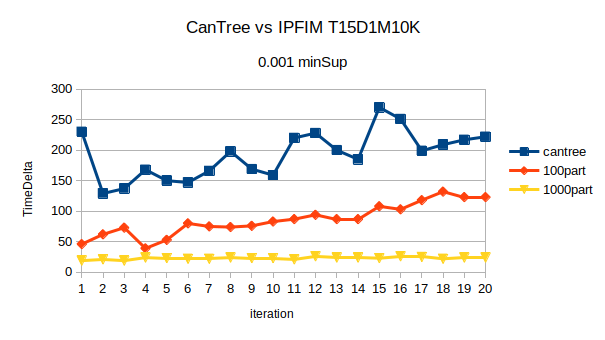
\includegraphics[width=\linewidth]{figures/IPFP1M0001}
  \caption{Inc. vs IPFIM}
  \label{fig:IPFP1M0001}
\end{figure}
Using 10M iterations and 100K itemsets with only 1 partition (regular CanTree), will result a memory issue with the used architecture, thus the results are not presented here. For a 1M transaction with 10K unique itemsets, the results improve at 5X for every 10X partitions. This is due to memory improvements and parallel computations.
For the Kosarak dataset, .

